\documentclass[12pt, a4paper]{article}


% A pretty common set of packages
\usepackage[margin=2.5cm]{geometry}
\usepackage[T1]{fontenc}
\usepackage{graphicx}
\usepackage{amssymb}
\usepackage{amsmath}
\usepackage{bm}
\usepackage{color}
\usepackage{float}
\usepackage{bm}
\usepackage{physics}
\usepackage{subcaption}

\DeclareRobustCommand{\uvec}[1]{{%
  \ifcsname uvec#1\endcsname
     \csname uvec#1\endcsname
   \else
    \bm{\hat{\mathbf{#1}}}%
   \fi
}}
\newcommand{\olsi}[1]{\,\overline{\!{#1}}} % overline short italic

\usepackage[colorlinks=true, 
    linkcolor=blue,          % color of internal links
    citecolor=blue,        % color of links to bibliography
    filecolor=blue,      % color of file links
    urlcolor=blue]{hyperref}

\title{[16-833] Homework 2 : Written Report}
\author{Bharath Somayajula}
\date{\today}

\begin{document}

\maketitle

\tableofcontents
\section{Theory}
\subsection{Q1}
The robot, starting at $\left[x_t, y_t, \theta_t\right]$ moves $d_t$ along the axis of the robot and then rotates by $\alpha_t$ radians in the counter-clockwise direction. This means that the displacements along $x$ and $y$ axes and change in orientation are
\[\Delta x_{t} = d_tcos(\theta_t)\]
\[\Delta y_{t} = d_tsin(\theta_t)\]
\[\Delta \theta_t = \alpha_t\]
This gives us
\[\Delta \mathbf{p}_t = [\Delta x_{t}, \Delta y_{t}, \Delta \theta_t]^T\]
Therefore the new pose is,
\[\mathbf{p}_{t+1} = \mathbf{p}_{t} + \Delta \mathbf{p}_t\] 
\[\mathbf{p}_{t+1} = \mathbf{p}_{t} + \left[d_tcos(\theta_t), d_tsin(\theta_t), \alpha_t\right]^T\] 

\subsection{Q2}
From the results in Q1, we know that
\[\mathbf{p}_{t+1} = \mathbf{p}_{t} + \Delta \mathbf{p}_t\]
Including the uncertainty in the moving mechanism, we get
\[\mathbf{p}_{t+1} = \mathbf{p}_{t} + \Delta \mathbf{p}_t + \mathbf{e}_t\]
This can be expanded as
\[\mathbf{p}_{t+1} = \begin{bmatrix}
  x_t + d_tcos(\theta_t) + e_xcos(\theta_t) - e_ysin(\theta_t)\\
  y_t + d_tsin(\theta_t) + e_xsin(\theta_t) + e_ycos(\theta_t)\\
  \theta_t + \alpha_t + e_{\alpha}\\
\end{bmatrix}\]
The equation above is non-linear. Moreover, the noise $\mathbf{e}_t$ is non-additive. This means the prediction step can be modeled as $\mathbf{p}_{t+1} = g(\mathbf{p}_t, \mathbf{u}_t, \mathbf{e}_t)$. Here, $\mathbf{p}_t = [x_t, y_t, \theta_t]^T$ and $\mathbf{e}_t = [e_x, e_y, e_{\alpha}]^T$ are groups of variables whose covariances are known\\\\
Therefore the covariance of $\mathbf{p}_{t+1}$ can be written as 
\begin{equation}
  \label{q2_1}
\Sigma_{t+1} = A\Sigma_tA^T + B\Sigma_{\mathbf{e}_t}B^T
\end{equation}
where $A$ and $B$ are Jacobian matrices and $\Sigma_{\mathbf{e}_t}=\begin{bmatrix}
  \sigma_x^2 & 0 & 0\\
  0 & \sigma_y^2 & 0\\
  0  & 0 & \sigma_{\alpha}^2\\
\end{bmatrix}$.\\\\
A and B can be computed as 
\[A = \begin{bmatrix}
  1 & 0 & -d_tsin(\theta_t)-e_xsin(\theta_t) - e_ycos(\theta_t)\\
  0 & 1 & d_tcos(\theta_t)+e_xcos(\theta_t)-e_ysin(\theta_t)\\
  0 & 0 & 1
\end{bmatrix} \text{ and } B = \begin{bmatrix}
  cos(\theta_t) & -sin(\theta_t) & 0\\
  sin(\theta_t) & cos(\theta_t) & 0\\
  0  & 0 & 1\\
\end{bmatrix}\]
Evaluating the Jacobians at $\mathbf{p}_t = [x_t, y_t, \theta_t]^T$ and $\mathbf{e}_t = [0, 0, 0]^T$, we get
\begin{equation}
  \label{q2_2}
A = \begin{bmatrix}
  1 & 0 & -d_tsin(\theta_t)\\
  0 & 1 & d_tcos(\theta_t)\\
  0 & 0 & 1
\end{bmatrix} \text{ and } B = \begin{bmatrix}
  cos(\theta_t) & -sin(\theta_t) & 0\\
  sin(\theta_t) & cos(\theta_t) & 0\\
  0  & 0 & 1\\
\end{bmatrix}
\end{equation}
We can estimate the overall covariance by substituting equations \ref{q2_2} in equation \ref{q2_1}.
\subsection{Q3}
Starting from pose $\mathbf{p}_t = \left[x_t, y_t, \theta_t\right]$, if $r_t$ and $\beta_t$ are range and orientations of the landmark, then the noise-free estimates of the location of the landmark are
\begin{equation}
  \label{q3_0}
  \mathbf{l} = \left[x_t + r_tcos(\theta_t + \beta_t), y_t + r_tsin(\theta_t + \beta_t)\right]^T
\end{equation}
where $\mathbf{p}_t = [x_t, y_t, \theta_t]^T$ and $\mathbf{z}_t = [\beta_t, r_t]^T$ are groups of variables with uncertainty.
Therefore, the overall uncertainty in the measurement of $\mathbf{l}$ is
\begin{equation}
  \label{q3_1}
  \Sigma_{\mathbf{l}} = C\Sigma_tC^T + D\Sigma_{\mathbf{z}}D^T
\end{equation}
  where $\Sigma_{\mathbf{z}} = \begin{bmatrix}
    \sigma_{\beta}^2 & 0\\
    0 & \sigma_r^2\\
  \end{bmatrix}$ $C$ and $D$ are Jacobian matrices that can be computed as
\[C = \frac{\partial \mathbf{l}}{\partial\mathbf{p}_t} \bigg\rvert_{\mathbf{p}_t=\mathbf{p}_t, \mathbf{z}_t=\mathbf{z}_t} \text{ and } D = \frac{\partial \mathbf{l}}{\partial\mathbf{z}_t} \bigg\rvert_{\mathbf{p}_t=\mathbf{p}_t, \mathbf{z}_t=\mathbf{z}_t}\]
Therefore,
\begin{equation}
  \label{q3_2}
C = \begin{bmatrix}
  1 & 0 & -r_tsin(\theta_t + \beta_t)\\
  0 & 1 & r_tcos(\theta_t + \beta_t)\\
\end{bmatrix} \text{ and } D = \begin{bmatrix}
  -r_tsin(\theta_t + \beta_t) & cos(\theta_t + \beta_t)\\
  r_tcos(\theta_t + \beta_t) & sin(\theta_t + \beta_t)\\
\end{bmatrix}
\end{equation}
We can estimate the overall covariance by substituting equations \ref{q3_2} in equation \ref{q3_1}.
\subsection{Q4}
From equation \ref{q3_0}, we geometry
\[r_tcos(\theta_t + \beta_t) = l_x - x_t \text{ and } r_tsin(\theta_t + \beta_t) = l_y - y_t\]
Squaring and adding the equations, we get
\[r_t^2 = (l_x - x_t)^2 + (l_y - y_t)^2\]
which translates into
\begin{equation}
  \label{q4_1}
  r_t = \sqrt{(l_x - x_t)^2 + (l_y - y_t)^2}
\end{equation}
and by dividing the equations and applying \textit{np.arctan2}, we get
\[\beta_t = \textit{np.arctan2}\left(\frac{l_y - y_t}{l_x - x_t}\right) - \theta_t\]
warping the angle, we get

\begin{equation}
  \label{q4_2}  
  \beta_t = \textit{warp2pi}\left(\textit{np.arctan2}\left(\frac{l_y - y_t}{l_x - x_t}\right) - \theta_t\right)
\end{equation}
Equations \ref{q4_1} and \ref{q4_2} give us a way to estimate measurements based on the robot state.\\\\
Therefore,
\begin{equation}
  \label{q4_3}
  \mathbf{z}_t = \begin{bmatrix}
    \textit{warp2pi}\left(\textit{np.arctan2}\left(\frac{l_y - y_t}{l_x - x_t}\right) - \theta_t\right)\\
    \sqrt{(l_x - x_t)^2 + (l_y - y_t)^2}\\
  \end{bmatrix}
\end{equation} 
\subsection{Q5}
The equation \ref{q4_3} is non-linear in $\mathbf{p}_t$ and $\mathbf{l}$ which means $\mathbf{z}_t = h(\mathbf{p}_t, \mathbf{l})$. Therefore, we need to linearize the equation by computing the Jacobians $\mathbf{H}_p$ and $\mathbf{H}_l$ where
\[\mathbf{H_p} = \frac{\partial \mathbf{h(\mathbf{p}_t, \mathbf{l})}}{\partial\mathbf{p}_t}\]
Computing the derivatives, we get
\[\mathbf{H_p} = \begin{bmatrix}
  \frac{l_y - y_t}{(l_x - x_t)^2 + (l_y - y_t)^2} & \frac{-(l_x - x_t)}{(l_x - x_t)^2 + (l_y - y_t)^2} & - 1\\
  \frac{-(l_x - x_t)}{\sqrt{(l_x - x_t)^2 + (l_y - y_t)^2}} & \frac{-(l_y - y_t)}{\sqrt{(l_x - x_t)^2 + (l_y - y_t)^2}} & 0\\
\end{bmatrix}\]
\subsection{Q6}
The Jacobian $\mathbf{H}_l$ can be written as
\[\mathbf{H_l} = \frac{\partial \mathbf{h(\mathbf{p}_t, \mathbf{l})}}{\partial\mathbf{l}}\]
Computing the derivatives we get
\[\mathbf{H_l} = \begin{bmatrix}
  \frac{-(l_y - y_t)}{(l_x - x_t)^2 + (l_y - y_t)^2} & \frac{l_x - x_t}{(l_x - x_t)^2 + (l_y - y_t)^2}\\
  \frac{l_x - x_t}{\sqrt{(l_x - x_t)^2 + (l_y - y_t)^2}} & \frac{l_y - y_t}{\sqrt{(l_x - x_t)^2 + (l_y - y_t)^2}}\\
\end{bmatrix}\]
We need not compute Jacobians w.r.t other landmarks i.e $\frac{\partial \mathbf{h(\mathbf{p}_t, \mathbf{l}_i)}}{\partial\mathbf{l}_j}$ since the measurements of landmarks are assumed to be independent of each other. Therefore such a Jacobian would be made of all zeros.


\section{Implementation and Evaluation}
\subsection{Q1}
The size of the landmark measurement vector is 12. Therefore, there are 6 landmarks.
\subsection{Q2}
\begin{figure}[H]
  \centering
  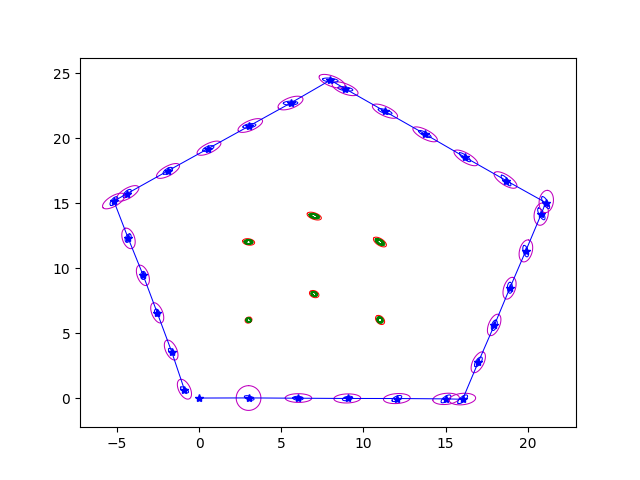
\includegraphics[width=1\textwidth]{./results/q2_2/result.png}
  \caption{Visualization with default settings}
\end{figure}

\subsection{Q3}
The EKF algorithm improves the estimation of trajectory in two steps. In the prediction step, the magenta ellipse is moved towards the true location but the uncertainty is still high given the relatively larger size of magenta ellipses. In the update step, this uncertainty is reduced based on measurements given the relatively small size of blue ellipses.\\\\
Similarly, the map is improved with time. This can be observed by noticing that the size of green ellipses reduces with time implying that evidence is accumulated and leading to a drop in uncertainty estimated by the EKF algorithm.
\subsection{Q4}
\subsubsection{Plot}
The ground truth locations are shown in cyan color. The marker has a non-zero radius and hence doesn't neatly fall inside the ellipses but the centers of the ground truth markers fall inside most of the ellipses estimated by the EKF algorithm which proves that EKF algorithm estimates are very close to the ground truth positions of landmarks.
\begin{figure}[H]
  \centering
  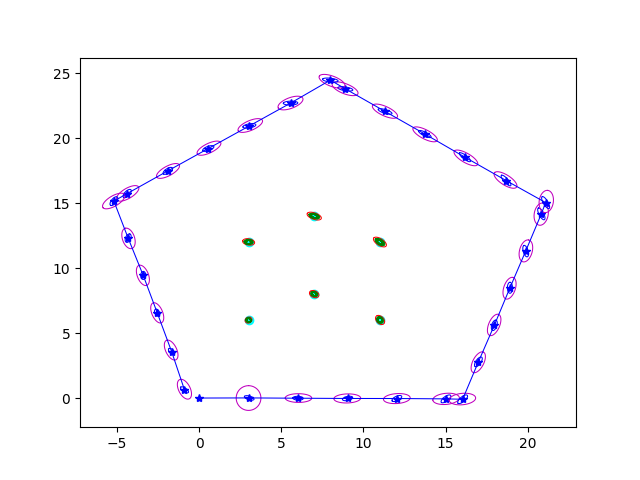
\includegraphics[width=1\textwidth]{./results/q2_4/result.png}
  \caption{Visualization of ground truth(in cyan)}
\end{figure}

\subsubsection{Metrics}
The table below summarizes the Euclidean and Mahalanobis distances for the 6 landmarks.
\begin{table}[H]
  \centering
  \begin{tabular}{|c|c|c|}
  \hline
  \textbf{Index} & \textbf{Euclidean Distance} & \textbf{Mahalanobis Distance} \\
  \hline
  1 & 0.00248222 & 0.00010843 \\
  2 & 0.00222136 & 0.00010859 \\
  3 & 0.00454603 & 0.00019824 \\
  4 & 0.00886395 & 0.00050701 \\
  5 & 0.0085716 & 0.00041845 \\
  6 & 0.00904752 & 0.00049835 \\
  \hline
  \end{tabular}
  \caption{Metrics for the landmarks}
  \end{table}
\noindent The absolute values of these numbers indicate that the EKF algorithm converged approximately to the true land landmark locations. The Mahalanobis distance differs from the Euclidean distance since it normalizes the error using the standard deviation. For example, in 1 dimension, the Mahalanobis distance measures $\frac{|x - \mu|}{\sigma}$ which is different from the Euclidean distance $|x - \mu|$.
\section{Discussion}
\subsection{Q1}
The zero-terms in the covariance matrix are non-zero by the end of the EKF algorithm due to the operations we perform in the update step where weupdate the covariance as $\Sigma_t = (I-K_tH_t)\bar{\Sigma}_t$. $K_t$ matrix is a dense matrix that informs ways in which various variables interact with each other. This causes output cross-covariances to be non-zero between various landmarks.\\\\
In the initial covariance matrix, there are two kinds of cross-covariances- the ones between pose parameters and landmark locations and the ones between various landmarks. We assumed that there are no cross covariances between pose and landmark locations. This is a reasonable assumption since the uncertainty in the initial robot location, which is potentially measured using a system such as GPS, is independent of the system used to measure the locations of key points. However, the assumption that the cross-covariances between various landmarks are zero is not reasonable since the locations of all landmarks are measured using the same method and therefore error in measurement of one landmark can lead to error in measurement of another landmark.
\subsection{Q2}
The plots below show the impact of increasing and decreasing each of the five parameters by a factor of 10.
\subsubsection{$\sigma_x$}

\begin{figure}[H]
  \centering
  \begin{subfigure}[b]{0.45\linewidth}
    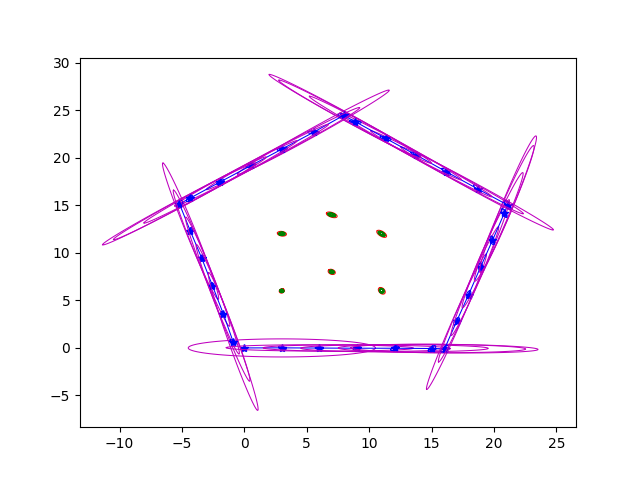
\includegraphics[width=\linewidth]{./results/q3_2/result_x.png}
    \caption{Increased by a factor of 10}
  \end{subfigure}
  \hspace{0.5cm}
  \begin{subfigure}[b]{0.45\linewidth}
    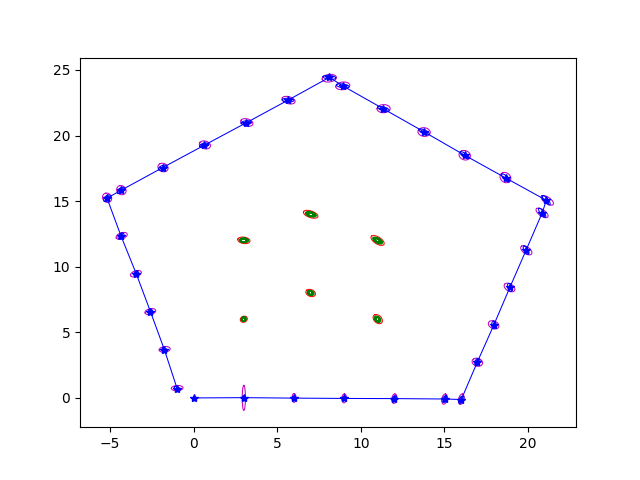
\includegraphics[width=\linewidth]{./results/q3_2/result_x_dec.png}
    \caption{Decreased by a factor of 10}
  \end{subfigure}
  \caption{Effect of changing $\sigma_x$}
\end{figure}
\subsubsection{$\sigma_y$}
\begin{figure}[H]
  \centering
  \begin{subfigure}[b]{0.45\linewidth}
    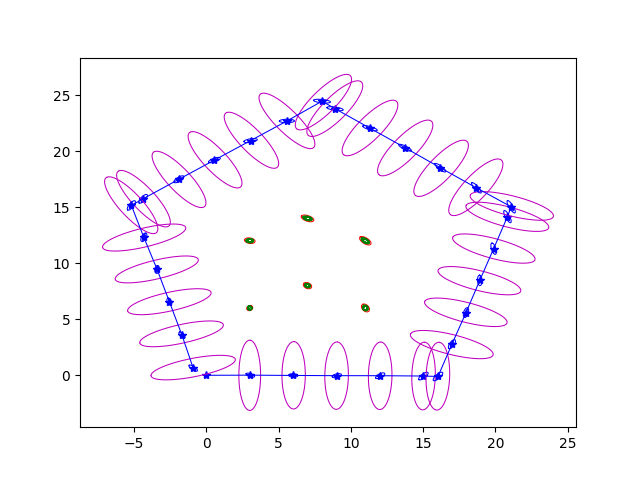
\includegraphics[width=\linewidth]{./results/q3_2/result_y.png}
    \caption{Increased by a factor of 10}
  \end{subfigure}
  \hspace{0.5cm}
  \begin{subfigure}[b]{0.45\linewidth}
    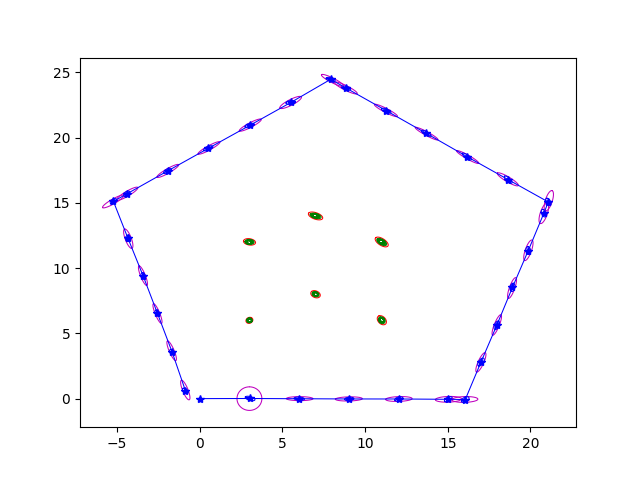
\includegraphics[width=\linewidth]{./results/q3_2/result_y_dec.png}
    \caption{Decreased by a factor of 10}
  \end{subfigure}
  \caption{Effect of changing $\sigma_y$}
\end{figure}
\subsubsection{$\sigma_{\alpha}$}
\begin{figure}[H]
  \centering
  \begin{subfigure}[b]{0.45\linewidth}
    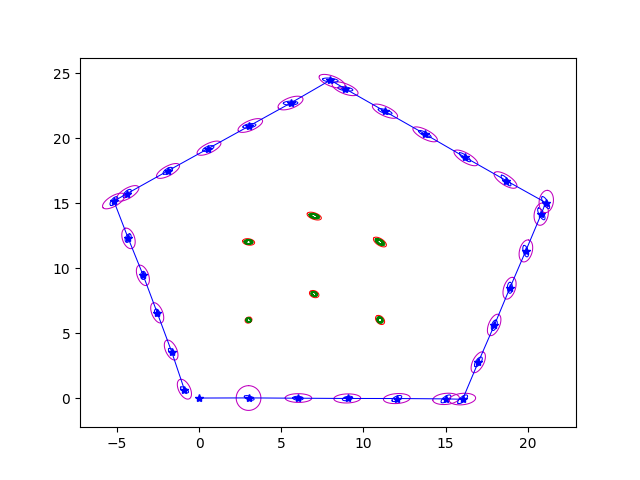
\includegraphics[width=\linewidth]{./results/q3_2/result_alpha.png}
    \caption{Increased by a factor of 10}
  \end{subfigure}
  \hspace{0.5cm}
  \begin{subfigure}[b]{0.45\linewidth}
    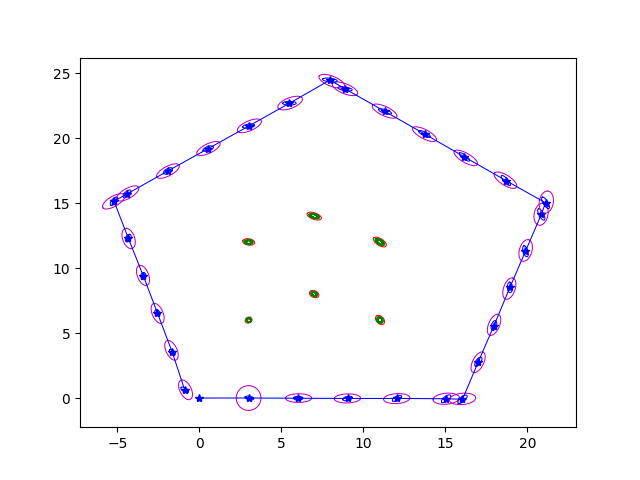
\includegraphics[width=\linewidth]{./results/q3_2/result_alpha_dec.png}
    \caption{Decreased by a factor of 10}
  \end{subfigure}
  \caption{Effect of changing $\sigma_{\alpha}$}
\end{figure}
\subsubsection{$\sigma_{\beta}$}
\begin{figure}[H]
  \centering
  \begin{subfigure}[b]{0.45\linewidth}
    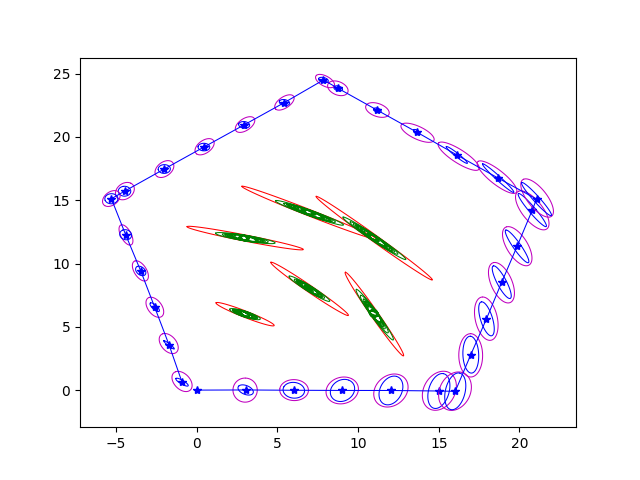
\includegraphics[width=\linewidth]{./results/q3_2/result_beta.png}
    \caption{Increased by a factor of 10}
  \end{subfigure}
  \hspace{0.5cm}
  \begin{subfigure}[b]{0.45\linewidth}
    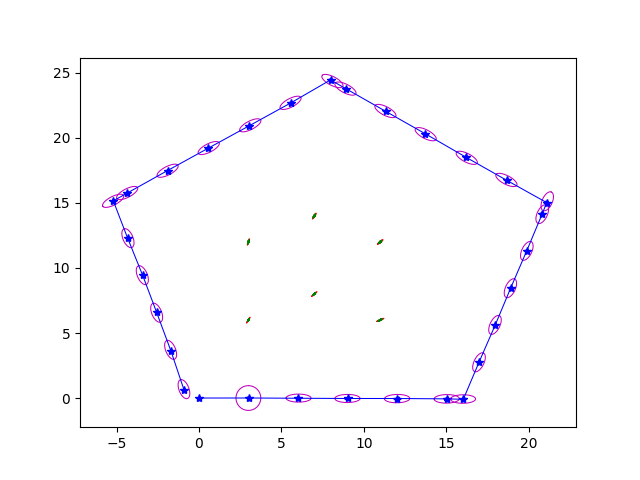
\includegraphics[width=\linewidth]{./results/q3_2/result_beta_dec.png}
    \caption{Decreased by a factor of 10}
  \end{subfigure}
  \caption{Effect of changing $\sigma_{\beta}$}
\end{figure}
\subsubsection{$\sigma_r$}
\begin{figure}[H]
  \centering
  \begin{subfigure}[b]{0.45\linewidth}
    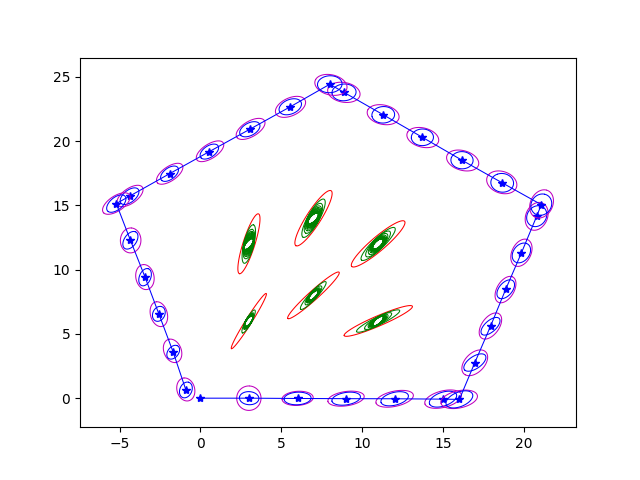
\includegraphics[width=\linewidth]{./results/q3_2/result_r.png}
    \caption{Increased by a factor of 10}
  \end{subfigure}
  \hspace{0.5cm}
  \begin{subfigure}[b]{0.45\linewidth}
    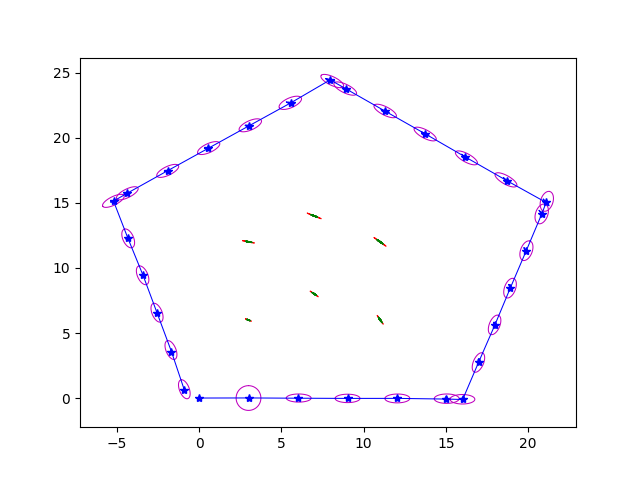
\includegraphics[width=\linewidth]{./results/q3_2/result_r_dec.png}
    \caption{Decreased by a factor of 10}
  \end{subfigure}
  \caption{Effect of changing $\sigma_r$}
\end{figure}
\subsubsection{Observations}
From the figures above, we can observe that increases in $\sigma_x$ and $\sigma_y$ lead to an increase in uncertainty of robot location along the x and y axes respectively which is clearly observed in the elongated sizes of ellipses drawn around the robot location in blue and green colors. Similarly, increases in $\sigma_{r}$ and $\sigma_{\beta}$  cause an increase in uncertainty of landmark location as seen by elongated red and green ellipses. Change in $\sigma_{\alpha}$ doesn't change the Visualization noticeably since robot orientation is not visualized in the 2D figure.\\\\
Decreasing the values by a factor of 10 has the opposite effect and uncertainties decrease as seen in the reduced sizes of ellipses in the figures above.
\subsection{Q3}
\begin{enumerate}
  \item The number of landmarks might increase unbounded in real-world problems but the number of \textit{visible} landmarks at any given instance is limited. Therefore, we can update the means and covariances of only the landmarks that are visible. This can significantly speed up the process.
  \item If the number of landmarks visible at any time step is too large, we can select top-k landmarks and update their means and covariances alone where k is a parameter that can be selected to manage computational resources. One metric that can be used to select top-k landmarks is to sort the landmarks based on covariances and select the landmarks with the greatest degree of uncertainty for updation. 
\end{enumerate}

\end{document}
